
\documentclass[12pt]{article}

\usepackage[utf8]{inputenc}
\usepackage[greek, english]{babel}

% Packages

\usepackage{alphabeta}
\usepackage{amsmath}
\usepackage{amsthm}
\usepackage{caption}
\usepackage{color}
\usepackage{fullpage}
\usepackage{graphicx}
\usepackage{latexsym}
\usepackage{listings}
\usepackage{pxfonts}
\usepackage{stackrel}
\usepackage{titlesec}
\usepackage{subfig}

% Commands
\newcommand{\R}{\mathbb{R}}
\newcommand{\N}{\mathbb{N}}
\newcommand{\norm}[1]{\left\lVert#1\right\rVert}
\newcommand{\margin}{\hspace{4pt}}
\newcommand{\centered}[1]{\begin{align*}#1\end{align*}}
\newcommand{\plot}[2]{\includegraphics{#1}\caption{#2}}
\newcommand{\code}[2]{\lstinputlisting[caption={#2}]{#1}}

% Environments
\newenvironment{rcases}
	{\left.\begin{aligned}}
	{\end{aligned}\right\rbrace}

\newenvironment{matlab}
	{\begin{figure}[hp]\centering\captionsetup{justification=centering}}
	{\end{figure}}

% Python Syntax Highlighting
\definecolor{string_color}{RGB}{0, 161, 13}
\definecolor{comment_color}{RGB}{46, 46, 46}
\definecolor{keyword_color}{RGB}{0, 112, 191}

\lstset{
    language=Python,
    captionpos=b,
    numbers=right,
    numberstyle=\small\ttfamily,
    frame=lines,
    showspaces=false,
    showtabs=false,
    breaklines=true,
    showstringspaces=false,
    breakatwhitespace=true,
    commentstyle=\color{comment_color}\textit,
    keywordstyle=\bfseries\color{keyword_color}\textbf,
    stringstyle=\color{string_color}\textit,
    morekeywords={self, lambda, __init__, __del__, __name__, for, in, not, and, or, :},
    basicstyle=\ttfamily,
    tabsize=4,
    keepspaces=true,
    columns=flexible
}

% Lengths
\setlength{\parindent}{0in}
\setlength{\oddsidemargin}{0in}
\setlength{\textwidth}{6.5in}
\setlength{\textheight}{10in}
\setlength{\topmargin}{-1.0in}
\setlength{\headheight}{18pt}

\titlespacing*{\subsection}
{0pt}{5.5ex plus 1ex minus .2ex}{4.3ex plus .2ex}

\title{\huge Examples of Linear Programming Problems\\Pattern Classification}
\author{Σιώρος Βασίλειος\\Ανδρινοπούλου Χριστίνα}
\date{Νοέμβριος 2019}

\begin{document}

\maketitle

\pagenumbering{gobble}

\pagebreak

\section{Introduction to Feature Vectors}

Έστω \textbf{m} αντικείμενα, τα οποία επιθυμούμε να ταξινομήσουμε σε δύο διακριτές ομάδες,
με κάθε αντικείμενο να ανήκει αυστηρά σε μία μόνο ομάδα. \\

Παραδείγματος χάριν \textbf{φυτά}, που επιθυμούμε να διαχωρίσουμε σε \textbf{εσπεριδοειδή} και \textbf{μη}.\\

Θεωρούμε πως τα αντικείμενα αυτά περιγράφονται επαρκώς από \textbf{n} το πλήθος χαρακτηριστικά. \\

Στην περίπτωση της ταξινόμησης φυτών, σε εσπεριδοειδή και μη, τα χαρακτηριστικά αυτά θα μπορούσαν
να είναι το \textbf{ύψος} του δέντρου, αν είναι \textbf{φυλλοβόλο} ή όχι, δηλαδή αν ρίχνει τα φύλλα του το χειμώνα και σε τι \textbf{κλίμα} ευδοκιμεί.

Μπορούμε λοιπόν, να αναπαραστίσουμε κάθε αντικείμενο με ένα \textbf{n}-διάστατο διάνυσμα. \\

Παραδείγματος χάριν, έστω ένα στιγμιότυπο \(x\) της κλάσης των εσπεριδοειδών με τα εξής \textbf{3} χαρακτηριστικά

\begin{align*}
    &\text{Ύψος : } \textit{8m} \\
    &\text{Φυλλοβόλο : } \textit{Όχι} \\
    &\text{Κλίμα : } \textit{Τροπικό} \vee \textit{Υποτροπικό} \vee \textit{Eύκρατο}
\end{align*}

τότε, το παραπάνω αντικείμενο μπορεί να αναπαρασταθεί από το \textbf{3}-διάστατο διάνυσμα

\centered{x^* = [\textit{8m}, \margin \textit{Όχι}, \margin \textit{Τροπικό} \vee \textit{Υποτροπικό} \vee \textit{Eύκρατο}]}

Είναι προφανές από το προηγούμενο παράδειγμα, ότι τα χαρακτηριστικά των αντικειμένων μπορεί να είναι μη αριθμητικά.
Ωστόσο, υπάρχουν μέθοδοι μετατροπής τους σε αριθμητικά κι ως εκ τούτου, το παραπάνω διάνυσμα μπορεί εύκολα να απεικονιστεί στον \( \R^{3} \).
Λοιπόν, θα εστιάσουμε στην περίπτωση των αριθμητικών χαρακτηριστικών. \\

\pagebreak

\section{Introduction to Pattern Classification}

Δεδομένης της προηγουμένως ορισθείσας αναπαράστασης αντικειμένων, θεωρούμε τα σύνολα

\begin{align*}
    K & = \{K_{1}, K_{2}, \dotsc , K_{l_k}\} & \text{ όπου }  K_i \in \R^{n} & \margin \forall i \in \lbrack 1, \dotsc l_k \rbrack \\
    N & = \{N_{1}, N_{2}, \dotsc , N_{l_n}\} & \text{ όπου }  N_i \in \R^{n} & \margin \forall i \in \lbrack 1, \dotsc l_n \rbrack
\end{align*}

Γνωρίζουμε ότι, ένα υπερεπίπεδο διαχωρίζει ένα αφινικό χώρο σε δύο ημιχώρους. \\

Τα σύνολα \(K\) και \(N\) χαρακτηρίζονται \textbf{γραμμικά} διαχωρίσιμα,
αν υπάρχει υπερεπίπεδο, τέτοιο ώστε τα αντικείμενα,
που ανήκουν στο σύνολο Κ να εντοπίζονται στον έναν ημιχώρο και τα αντικείμενα,
που ανήκουν στο σύνολο N στον άλλον ημιχώρο. \\

Πιο τυπικά θα λέγαμε ότι τα σύνολα Κ και N χαρακτηρίζονται \textbf{γραμμικά} διαχωρίσιμα,
αν υπάρχουν \( a \in \R^{n} \) και \( b \in \R \), τέτοια ώστε

\begin{align*}
    K & \subseteq \{ x \in \R^{n} : a^{T} \cdot x \geq b \} \\
    N & \subseteq \{ x \in \R^{n} : a^{T} \cdot x < b\}
\end{align*}

\begin{figure}[hp]
    \centering
    \subfloat[Γραμμικά διαχωρίσιμα σύνολα]{{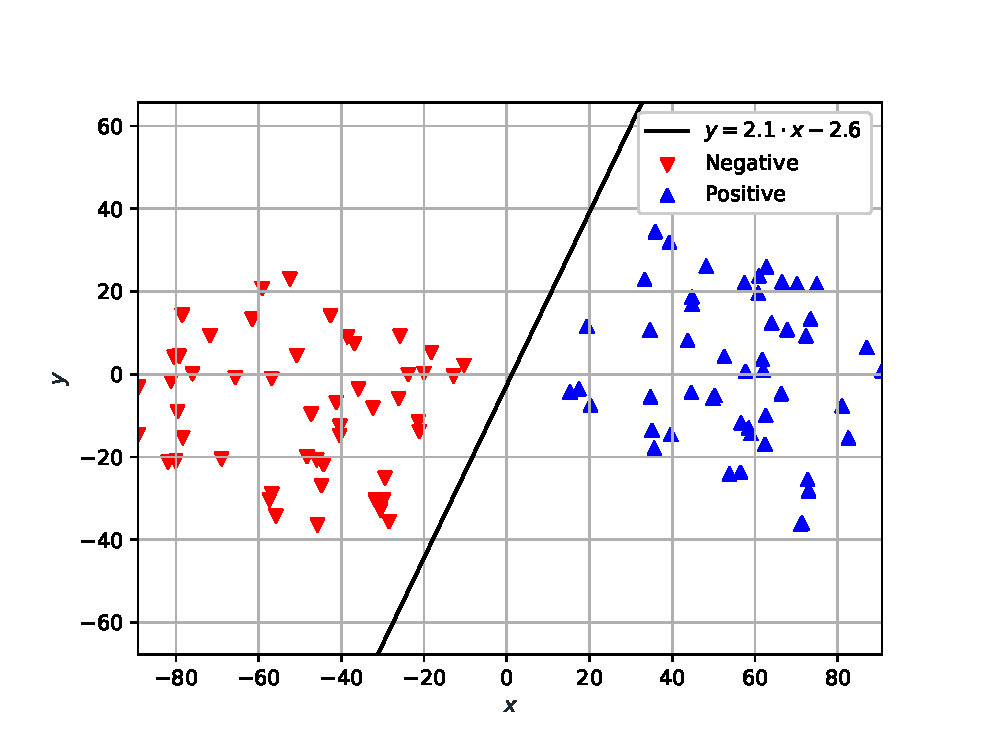
\includegraphics[width=7.5cm]{linearly_separable}}}
    \qquad
    \subfloat[Μη γραμμικά διαχωρίσιμα σύνολα]{{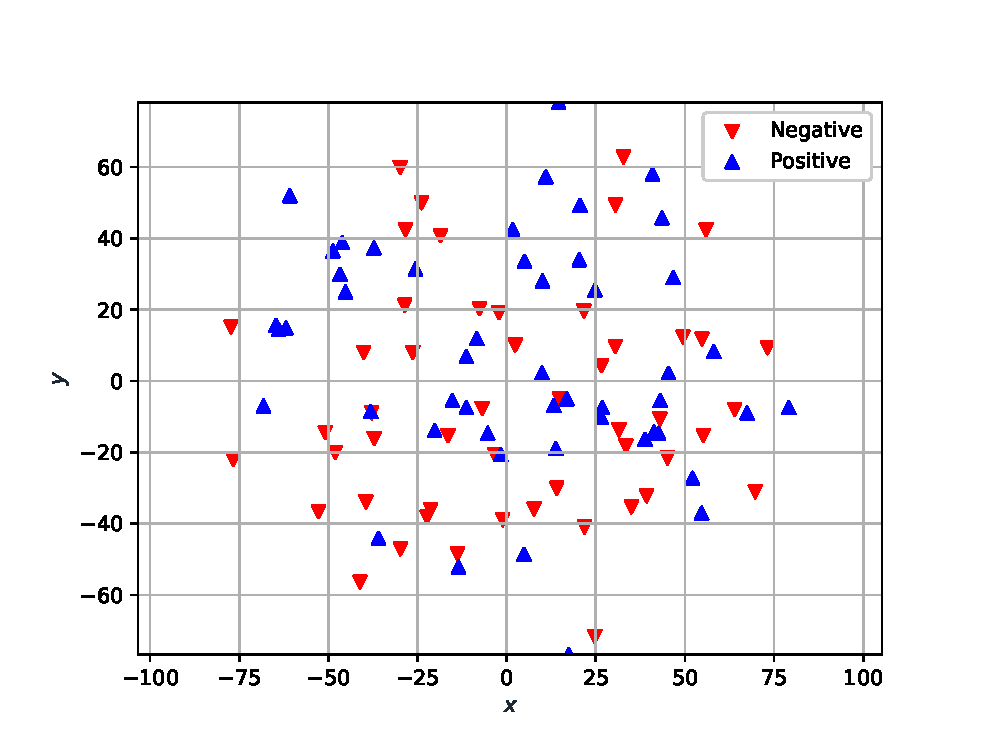
\includegraphics[width=7.5cm]{not_linearly_separable}}}
\end{figure}

\pagebreak

\section{Pattern Classification via Linear Programming}

% Ayto kanto oti 8es, balto opou tairiazei edw mesa h an dn tairiazei ka8olou bgalto plhrws
% Isws sto telos kserw gw gia dieukrinhsh prin to modeling s python i guess

Ένας γραμμικός ταξινομητής αρχικά τροφοδοτείται με ένα σύνολο αντικειμένων,
η κλάση των οποίων είναι γνωστή, εκ των προτέρων.
Βάσει αυτού του συνόλου υπολογίζονται τα \( a \in \R^{n} \) και \( b \in \R \).
Το σύνολο αυτό αποτελεί το σύνολο εκπαίδευσης του ταξινομητή. \\

Για κάθε αταξινόμητο αντικείμενο \( x \), το πρόσημο της παράστασης \( a^{T} \cdot x - b \)
υποδεικνύει σε ποια ομάδα ανήκει. \\

\pagebreak

\section{Coding}



\end{document}
